% !TEX root = ../my-thesis.tex
%

\chapter{Visualization Concepts}
\label{sec:visualconcepts}

In this chapter we start by giving an introduction to the main framework used in our application, three.js, followed by an explanation of the core visualisation concepts used in the project. We are also going to explain why we chose three.js over WebGL for our project by constructing and analysing a small demo for both frameworks. The task in the demo is to visualise a coloured and rotating three-dimensional cube. Each major concept mentioned in this chapter is incorporated in the demo. We will refer back to it at the end of each section and illustrate the differences between the two frameworks. This way we want to illustrate why three.js is the better choice for developing a molecule visualisation application. The demo code can be found in our project repository at \url{https://gitlab.rlp.net/ppfannes/bachelor_thesis/-/tree/develop/Research/thesis_examples}.

\section{three.js}
\label{sec:visualconcepts:three}

three.js (formerly known as three.as) is a multi-purpose, open-source 3D JavaScript library written by mrdoob. The aim of three.js is to pose as a general framework for 3D tasks such as visualisation, animation and many more \cite{mrdoob2022Oct}. Additionally, each functionality or component should be designed in a way that does not rely on third-party libraries. In order to achieve those goals three.js is easily extensible in case a new way of rendering is discovered or new components have to be added. As such it provides basic implementations of mathematical structures needed like vectors, matrices as well as other core features for visualisation like Buffers, Objects, Geometries and Uniforms. In addition there are also features for animating, file and object loading, integrating audio tracks and many more. 

To take a closer look at how visualisation works in three.js we will inspect the piece of code shown in snippet \ref{sec:visualconcepts:three:toyscene}.

\begin{listing}[H]
	\begin{minted}[autogobble, bgcolor=bg, breaklines, linenos]{javascript}
	const scene = new THREE.Scene();
	const camera = new THREE.PerspectiveCamera(75, window.innerWidth / window.innerHeight, 0.1, 1000);

	const renderer = new THREE.WebGLRenderer();
	renderer.setSize(window.innerWidth / window.innerHeight);
	document.body.append(renderer.domElement);

	const geometry = new THREE.BoxGeometry(1, 1, 1);
	const material = new THREE.MeshBasicMaterial({color: 0x00FF00});
	const cube = new THREE.Mesh(geometry, material);
	scene.add(cube);

	camera.position.z = 5;

	function animate() {
		requestAnimationFrame(animate);
	
		cube.rotation.x += 0.01;
		cube.rotation.y += 0.01;
	
		renderer.render(scene, camera);
	};

	animate();
	\end{minted}
	\caption{Creation of a small scene in three.js. The scene contains a rotating and coloured cube.}
	\label{sec:visualconcepts:three:toyscene}
\end{listing}
Setting up visualisation in three.js works by first creating a \textit{Scene} and \textit{Camera} object. The \textit{Scene} acts as a container where all the objects that should be rendered will be added to. The \textit{Camera} defines the field of view in which you can see the rendered objects. Next up is the initialisation of the renderer used, in this case a \textit{WebGLRenderer}. It acts as an API which abstracts away most of WebGL's functionalities and leaves the user with a set of core functions to render objects. This allows developers to focus more on the development of their application instead of having to invest a decent amount of time creating visualisations with purely WebGL. Especially if the project features various representations of objects as it is the case with our \textit{Molecule Visualizer}. After the renderer has been initialised the cube will be created in lines 8-10. In three.js objects are represented as meshes that consist of a Geometry describing the shape of the object and a material describing its outward appearance. The cube is then added to the \textit{Scene} and is now ready to be rendered which will be done in the animate function. Lines 16-19 make the cube rotate around the x and y-axis while the actual rendering takes place in line 21. Using the \textit{Scene} and the \textit{Camera} the renderer visualises the cube on the screen within the field of view of the camera. To actually see the output of this code it has to either be embedded into an HTML file directly or you need to reference the source file containing the code. Both methods are shown in snippet \ref{sec:visualconcepts:three:threeembedding}.

\begin{listing}[H]
	\begin{minted}[autogobble, bgcolor=bg, breaklines, linenos]{html}
	<!-- Method 1: Embed source code directly into the HTML page. -->
	...
	<script src="path/to/three.js"></script>
	<script>
		<!-- visualisation code here... -->
	</script>
	...
	
	<!-- Method 2: Specify path to the source code file. -->
	...
	<script src="path/to/visualisation/source/file"></script>
	...
	\end{minted}
	\caption{Methods of embedding three.js code into a web page to see the visualisation.}
	\label{sec:visualconcepts:three:threeembedding}
\end{listing}

\section{Meshes}
\label{sec:visualconcepts:meshes}

Meshes are used to model complex structures like living beings or geometrical objects. They are constructed by approximating the surface of objects using triangles. Instead of calculating them directly while rendering they are implicitly defined via the positions of their corners, also called vertices. The connection between a pair of vertices is called edge and they are used to keep track of all vertices that make up a triangle, also called face. Those three components, vertices, edges and faces, are the main components that construct a mesh. Additionally you can also define further properties that change the appearance of the mesh like materials or UV Coordinates. During the render pipeline in the graphics hardware shaders are used to help building a concrete mesh. Materials define regions in the mesh that use a different shader than the rest which results in a changed appearance of the area. UV Coordinates also influence the later outward appearance of a mesh by specifying which parts of a two-dimensional texture map are applied to which part of a mesh. UV Coordinates can be considered a mapping of the two-dimensional texture space to the three-dimensional coordinate space of the mesh. Each vertex is assigned a pixel of the texture map that will later be rendered on the vertex's position.

\begin{listing}[H]
\begin{minted}[autogobble, bgcolor=bg, breaklines, linenos]{javascript}
// WebGL mesh creation.
...
function initBuffers(gl) {
	const posBuffer = gl.createBuffer();
	gl.bindBuffer(gl.ARRAY_BUFFER, posBuffer);
	const vertices = [...];
	gl.bufferData(gl.ARRAY_BUFFER, new Float32Array(vertices), gl.STATIC_DRAW);
	...
	const colBuffer = gl.createBuffer();
	gl.bindBuffer(gl.ARRAY_BUFFER, colBuffer);
	gl.bufferData(gl.ARRAY_BUFFER, new Float32Array(colors), gl.STATIC_DRAW);
	
	const indBuffer = gl.createBuffer();
   	gl.bindBuffer(gl.ELEMENT_ARRAY_BUFFER, indBuffer);
   	const indices = new Uint16Array([...]);
   	gl.bufferData(gl.ELEMENT_ARRAY_BUFFER, indices, gl.STATIC_DRAW);
   	...
}
...
\end{minted}
\begin{minted}[autogobble, bgcolor=bg, breaklines, linenos]{javascript}
	// three.js mesh creation.		
	const boxGeometry = new THREE.BoxGeometry(boxWidth, boxHeight, boxDepth);
	const boxMaterials = [...];   // Array of MeshBasicMaterial instances.
	const box = new THREE.Mesh(boxGeometry, boxMaterials);
\end{minted}
\caption{Mesh creation in WebGL vs. three.js. WebGL needs to initialise buffer objects for vertex positions, colors and face indices and bind them in order to prepare a mesh. three.js only has to create instances for the object's geometry and material to create meshes.}
	\label{sec:visualconcepts:meshes:meshinitex}
\end{listing}

To get a better understanding of how mesh creation works we will take a look at how both WebGL and three.js handle this task. The code snippets in listing \ref{sec:visualconcepts:meshes:meshinitex} show the process of mesh creation for WebGL and three.js respectively. As one can see, it takes farm more lines of code (LOC) to produce a mesh in WebGL than in three.js. To be able to create a mesh in WebGL you need to first define the positions of the vertices followed by the colours of the various Faces. Both the positions and colours are then bound to buffer objects which will allow WebGL to pass multiple values to the shaders during rendering. The last step is the creation of an index array which defines the vertices that make up a face.

Defining a mesh in three.js only requires the geometry of the object and the material used to alter its appearance which are already provided as base classes, \textit{BufferGeometry} and \textit{Material}. \textit{BufferGeometries} act as a container for different attributes regarding meshes like Vertex positions, Face normals or UV Coordinates as well as custom attributes. Attributes are stored similarly to WebGL. Lines 7, 11 and 16 show that the attribute information is stored by writing it to the corresponding buffer that was bound previously using \textit{gl.bindBuffer}. The arrays have to be converted to typed JavaScript arrays before they can be saved. Instead of only using typed JavaScript arrays \textit{BufferGeometries} use a wrapper class and the corresponding typed array to store attribute information (e.g. \textit{Float32BufferAttributes} for \textit{Float32Arrays}). In the case of the \textit{BoxGeometry} class according to the width, height and depth provided in the constructor the geometry of a box with those parameters will be created in the background. \textit{Materials} contain information regarding the appearance of the object to be rendered. Attributes are stored as properties of the \textit{Material} instance to keep it independent from the renderer framework used. The \textit{Mesh} class ultimately acts as a container for both the geometry information as well as the appearance information of objects. Compared to WebGL, three.js abstracts away the creation of geometry attributes and material properties by introducing classes that handle these tasks upon instantiation.

\section{Camera}
\label{sec:visualconcepts:camera}

In order to visualise the mesh of a three-dimensional object as a two-dimensional image its vertex coordinates need to be transformed. This transformation is referred to as \textit{Projection} and describes the process of mapping the vertex positions to points within the two-dimensional image plane. A series of matrix multiplications is used to transform vertex coordinates where each matrix plays a different role during transformation. This can be seen in figure \ref{sec:visualconcepts:camera:transform}. The first step involves transforming the vertex coordinates from object to world space using the model matrix. It is able to manipulate objects by altering their position, rotation and size. After that the world space coordinates need to be transformed with respect to the camera. This is achieved by applying the view matrix which can be expressed as the inverse of the camera's model matrix. The final transformation step involves the projection matrix which contains information about the camera's field of view. Applying the projection matrix ensures that only coordinates within the camera's field of view will be rendered, effectively discarding all other coordinates. There are two types of projection matrices, each yielding a different result when applied. The perspective projection matrix creates an output that is similar to how the human eye perceives objects. The further away an object is the smaller it will be rendered. Applying an orthographic projection matrix yields an image that has no depth information at all. Every object in the field of view of the camera will appear to have the same depth value. The figure also shows that some steps can be combined to gain performance by applying less matrix multiplications.

\begin{figure}[htb]
	\centering
	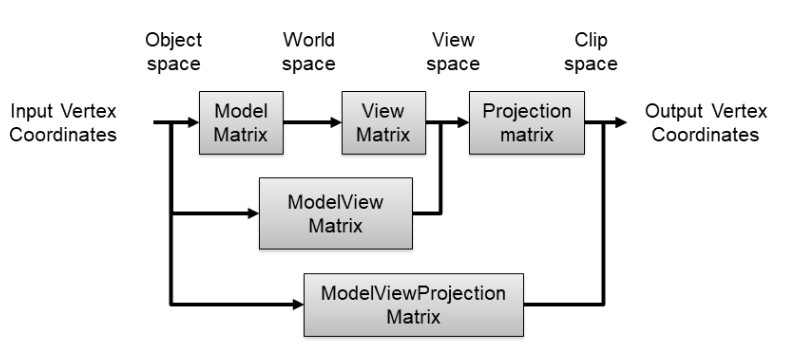
\includegraphics[width=\textwidth]{gfx/transformations.jpg}
	\caption[Transformation of vertex coordinates to image plane coordinates.]{Transformation of vertex coordinates to image plane coordinates\footnotemark.}
	\label{sec:visualconcepts:camera:transform}
\end{figure}
\footnotetext{https://www.doc.ic.ac.uk/~bkainz/graphics/notes/GraphicsNotes0405.pdf; accessed on 31 October 2022}

Listing \ref{sec:visualconcepts:camera:cameraex} shows how the camera is manipulated in WebGL and three.js. The projection matrix has to be explicitly created in WebGL by first defining the fov, aspect ratio, near and far plane and then applying those values on an empty matrix (lines 5-11). The model-view Matrix is treated similarly. First you create an empty matrix and the you apply the transformations on it that will alter the object's position and rotation during rendering. For the transformations to take effect, the matrices need to be stored in their respective Uniforms so the shaders have access to them. In three.js you create an instance of the \textit{PerspectiveCamera} class in order to manipulate objects. The parameters passed to its constructor are the same that are used to create the projection matrix in WebGL. Instead of directly working with the matrices, you manipulate the object directly and inside the \textit{renderer.render} function the Projection and model-view matrices will be updated. This approach seems a bit more intuitive, because you apply the transformation directly to the object and the matrices are updated during rendering instead of the other way around like WebGL does. You can also see that everything regarding the matrices which transform objects is abstracted away through the \textit{renderer.render} function.

\begin{listing}[H]
\begin{minted}[autogobble, bgcolor=bg, breaklines, linenos]{javascript}
// WebGL camera.
...
function sceneDraw(gl, progInfo, buffers, deltaTime) {
	...
    glMatrix.mat4.perspective(projMatrix, fov, aspect, near, far);

    const modelViewMatrix = glMatrix.mat4.create();
    glMatrix.mat4.translate(modelViewMatrix, modelViewMatrix, new Float32Array([0.0, 0.0, -4.0]));
    glMatrix.mat4.rotateZ(modelViewMatrix, modelViewMatrix, cubeRotation);
    glMatrix.mat4.rotateY(modelViewMatrix, modelViewMatrix, cubeRotation * 0.7);
    glMatrix.mat4.rotateX(modelViewMatrix, modelViewMatrix, cubeRotation * 0.3);
   	...
   	gl.uniformMatrix4fv(progInfo.uniformLocs.projMatrix, false, projMatrix);
    gl.uniformMatrix4fv(progInfo.uniformLocs.modelViewMatrix, false, modelViewMatrix);
   	...
}
...
\end{minted}
\begin{minted}[autogobble, bgcolor=bg, breaklines, linenos]{javascript}
// three.js camera.		
const camera = new THREE.PerspectiveCamera(50, canvas.clientWidth / canvas.clientHeight, 0.1, 100);
camera.position.z = 3.5;
...
time *= 0.001;
    
box.rotation.z = time;
box.rotation.y = time * 0.7;
box.rotation.x = time * 0.3;
    
renderer.render(scene, camera);
...
\end{minted}
\caption{Camera manipulation in WebGL vs. three.js. While you have to directly change the projection and model-view matrix in WebGL you only have to transform objects in three.js The camera will be adjusted in the \textit{renderer.render} function.}
\label{sec:visualconcepts:camera:cameraex}
\end{listing}

\section{Raycasting}
\label{sec:visualconcepts:raycasting}

As the name implies \textit{Raycasting} uses rays that are cast from the focal point to detect and render objects. For every pixel that will be generated on the Image Plane a ray is generated and traced until all intersections with objects in the world space are found. The first intersection found determines which object will be rendered on the corresponding pixel of the image plane. Another useful application of \textit{Raycasting} is \textit{object picking}. By casting the ray from the mouse pointer's position instead of the focal point and stopping after finding the first intersection one can determine if the mouse pointer is currently hovering over an object.

\section{Virtual Reality}
\label{sec:visualconcepts:virtualreality}

\textit{Virtual Reality} (VR) is the simulation of a world either similar to the real world or different from it. VR offers various degrees of immersion into the simulated surroundings such as visual immersion, motion tracking or full body immersion \cite{10.3389/fpsyg.2018.02086}. There are several types and methods as well including simulation-based, projector-based, desktop-based or VR via head-mounted devices (HMD). Projector-based simulations are used for applications in which it is necessary to have an accurate and realistic representation of the real world. Examples would be construction modelling, robot navigation or airplane simulation. Whereas in simulation-based VR the surroundings rendered can be made-up.  The key point is generating an experience as if the user is truly present in the virtual world by providing realistic feedback based on the user's inputs. This can be seen in many simulation games where one is driving a vehicle or operating a machine. Desktop-based VR involves displaying a three-dimensional world on a regular display without the use of other devices connected to VR such as lenses or motion-tracking devices. Instead the feeling of immersion is created by using various triggers or responsive characters. HMDs consists of two small displays inside the device that render the environment for each eye separately. This enables stereoscopic vision that results in a more realistic experience of the surroundings. A binaural sound system as well as motion tracking of the head enhance this experience even further. Motion controls or an omnidirectional treadmill to allow for realistic movement and interactions within the virtual world are optional.

Incorporating VR into web applications poses a problem, because of the wide range of devices on the market all supporting different degrees of movement, controls and position tracking. That is why in 2016 \textit{WebVR} was introduced as a first attempt of creating a general API for web based VR applications \cite{BibEntry2018Sep, WebVRIntro}. It featured full support for VR headsets, motion and position tracking as well as a Gamepad interface for controller support. WebVR made it possible to more easily develop VR applications without the developers being concerned about supporting multiple devices, because it serves as an abstraction of the devices' hardware. While it posed as a great start to web-based VR development it was only an experimental API and it soon became apparent that a new framework needed to be created. This led to the introduction of \textit{WebXR} two years later in 2018 \cite{BibEntry2022Jul}. One key difference is the support for \textit{Extended Reality} (XR) meaning Augmented Reality (AR) and VR. Another difference is the controller support for some VR devices. Instead of leveraging the existing Gamepad interface WebXR offers an own implementation along with events that are responsible for squeeze and select controls.

All applications build with the WebXR API follow a similar life cycle \cite{BibEntry2022Aug}. The first code snippet in listing \ref{sec:visualconcepts:virtualreality:vrex} illustrates said cycle and how it can be implemented in WebGL. At first you have to request a session from \textit{navigator.xr} and set the mode in which the VR session should be started in. After the session has been set successfully, the returned Promise will be resolved in which the \textit{xrReferenceSpace} will be set up. The reference space is responsible for setting up the movement tracking environment within a VR scene. There are different modes for the \textit{xrReferenceSpace} which make assumptions about the user's movement from the initial starting point in the scene as well as in the environment in general and thus adjust the stability of the tracking space. Then you need to make sure that the WebGL context used to render the normal scene is now set up to render the VR environment. This is done by calling \textit{gl.makeXRCompatible}. Once the render context is updated you need to update the render state and frame buffer as well. Doing so will tell the WebXR API where to render the contents of the VR scene to. Now that the set up for the \textit{xrSession} is complete the only thing left is to set up a render loop for the scene. The callback is defined similarly to a normal scene with the exception that it now also takes a second parameter which is an \textit{xrFrame}. The \textit{xrFrame} object is responsible for saving the state of all tracked objects within a VR scene. You are able to retrieve the viewer pose from an \textit{xrFrame} which is needed for rendering the scene to both lenses of an HMD. By calling \textit{xrSession.requestAnimationFrame} you register the render callback in the same way as in a non-VR scene.

The rendering process of a VR scene is similar to that of a non-VR one with the exception that the scene has to be rendered multiple times, one for each view matrix in the viewer pose. Each view matrix represents the transformations associated with the lens of a VR device and the Projection as well as the Model-View Matrix are constructed with respect to it (lines 27 and 28 of the first snippet). To ensure that the scene has been rendered for all devices registered in the \textit{xrSession}, \textit{gl.finish} is called in line 22 of the first snippet. This function waits until all previously called WebGL functions have been completed.
The above process has been drastically abstracted in three.js as seen in code snippet two. In order to create a VR scene one has to import the \textit{VRButton.js} file which initiates the \textit{xrSession} after being clicked. Then you need to tell the renderer you want to enable VR by setting the \textit{renderer.xr.enabled} flag to \textit{true}. \textit{renderer.xr} is an instance of the WebXRManager class which manages essentially everything about the VR environment, e.g. session set-up, input devices, device cameras or updating of components during VR rendering. To create the animation loop in three.js you call the \textit{renderer.setAnimationLoop} method and provide the render function as an argument. \textit{setAnimationLoop} accomplishes the same result as \textit{xrSession.requestAnimationFrame} by registering the render function within the \textit{WebXRManager} to be called during visualisation. 
When dealing with VR applications three.js provides an API that abstracts a big part of the set-up usually needed for them. As one can see in the first code snippet, you would normally need to set up the entire session as well as the render environment yourself while in three.js you only need a few small changes to the source code to create a stable VR application. 
\begin{listing}[H]
\begin{minted}[autogobble, bgcolor=bg, breaklines, linenos]{javascript}
// WebGL VR scene.
...
function enterVR() {
	navigator.xr.requestSession('immersive-vr').then((session) => {
	// Set up xrReferenceSpace.
	inVR = true;

	gl.makeXRCompatible().then((xrContext) => {
		// Set up render state and frame buffer.
	});

	const renderVR = (now, frame) => {
		// Similar to render with the exception of setting up xrFrame; call to sceneDrawVR with same parameters as in non-VR.
	};

	xrSession.requestAnimationFrame(renderVR);
	});
}
...
function sceneDrawVR(gl, progInfo, buffer, deltaTime) {
	// Same setup as in sceneDraw; retrieve pose of xrFrame so you can render the scene for each eye of the VR headset.
	gl.finish();
}
...
function renderEye(gl, progInfo, buffers, eye) {
	// Set up Projection and View Matrix with respect to the eye that is currently rendered; rest of function like sceneDraw.
	projection = eye.projectionMatrix;
	view = eye.transform.inverse.matrix;
	...
}
...
\end{minted}
\begin{minted}[autogobble, bgcolor=bg, breaklines, linenos]{javascript}
// three.js VR scene.
// import VRButton.js for setting up xrSession.
...
renderer.xr.enabled = true;
document.body.appendChild(VRButton.createButton(renderer));
...
renderer.setAnimationLoop(render);
\end{minted}
\caption{VR setup in WebGL vs three.js. A lot of setup is required in order to set up a VR scene for WebGL. All the functionality for setting up VR in three.js is abstracted away in \textit{VRButton} and \textit{renderer.xr}.}
\label{sec:visualconcepts:virtualreality:vrex}
\end{listing}